

%************************Document class********************************************
% Define document class with options
% Available font size: 10pt, 11pt, 12pt
% Default options: 11pt, a4paper, onecolumn, onside, final
%************************************************************************************

\documentclass{chart}
%\documentclass[twocolumn]{chart}

% ****************** packages*******************************************************
% following packages are already added 
% ams, xcolor, caption, subcaption, booktabs, footmisc, microtype, graphicx, 
% appendix, geometry, natbib 
%************************************************************************************

%************************Font setting************************************************
% Add the packages at this place
% Default font: `txfonts' which is one of the 'times' fonts
% Remove the below package and add the font package which you like
%************************************************************************************

\usepackage[varg]{txfonts} 
\usepackage[skip=10pt plus1pt, indent=40pt]{parskip}


%**************Line spacing, page margins, and graphics*****************************
% Default line spacing for abstract and references is one, and for sections, it is 1.33
% Change line spacing with '\linespacing[]', 
% e.g., \linespacing[1.66] for doublespacing
% Default page margin: top=bottom=left=right= 2 cm   
% Change default margin with the `\geometry' command 
% Graphics path can be set if images are in separate folder
%**********************************************************************************

%\geometry{margin=2.5cm}

\graphicspath{{Images/}}  

%***********************Bibliography********************************************** 
% Default reference style is 'rsc'
% For citation styles, use'\citestyle[options] command
% Available options: numbers, sort&compress, super, square, authoryear, etc.
%*********************************************************************************

%\citestyle[authoryear]
\refstyle{rsc}

%*********************User defined macros/packages********************************
% Define the required newcomands/renewcomands/renewenvironments
% Change abstract color with '\abscolor{backgroundcolor}' command
% Any other document setting
%*********************************************************************************

%\abscolor[linecolor=red]{backgroundcolor=yellow!10} 
%\hypersetup{hidelinks}

%%************************ Details for title page********************************
% Provide the information about title, author, date, email, and address
% Enable \chcopyright[], if you want to suppress the copyright information
%*********************************************************************************

\date{2023}
\Email{akhilareddy954@gmail.com}

%\chcopyright[] 

%%***************************** Main body*****************************************
% Main body starts from \begin{document} command
%*********************************************************************************

\begin{document} 
\begin{titlepage}
 \begin{center}
 \vspace*{1cm}

       \textbf{BALANCING EVERYDAY TASKS AND PROJECT MANAGEMENT WITH EASE}

       \vspace{0.5cm}
        A Project Report\\
Submitted in partial fulfillment of the requirements\\ for
the Software Project Management\\

 \vspace{1cm}
        Master of Technology\\
in\\
Department of Applied Computer Science\\
\vspace*{1cm}
        by\\
       \vspace*{1cm}

        AKHILA JAKAMUKALA (40277133)\\
     under the supervision of\\
	 P. KAMTHAN\\
	Professor

            
       \vspace{1.5cm}
              
   \end{center}
\end{titlepage}

 \begin{center}
\textbf{ABSTRACT}
\end{center}
 \hspace{1cm}Project management is the discipline of planning, organizing, securing, managing, leading, and controlling resources to achieve specific goals. The major challenges of project management include unrealistic deadlines, a lack of communication, unclear dependencies, an inability to manage risk, a lack of unobstructed vision and goals. It is tough to meet these hurdles, and often the project fails due to not meeting these challenges. When project dispersion is higher, the problem is significantly worse. Without the proper guidance, estimating daily effort or reallocating resources can be difficult and causes action from the project lead. Developing effective guidelines, creating an intuitive depiction of the project structure, managing resources and time, and showing more effective dispute resolution strategies are only a few of the difficulties met in resource and project management. Coordination of several project components is necessary for software project management to produce a successful outcome. \\
 	            
\begin{keywords}
\textit{ Project management,  dependencies, Reallocating resources, Prioritization, Planning, Organizing.}
\end{keywords} 
	
\newpage
 \vspace*{0.5cm}
            
\tableofcontents 
\listoffigures          
%================================Mainmatter=========================================
\newpage
  \vspace*{0.5cm}
\section{Introduction}\label{sec:intro}  
\hspace{1cm} In today's fast-paced world, managing daily tasks while simultaneously handling project-related tasks is a crucial skill. However, the balancing act between routine tasks and project work often results in a decrease in productivity due to a lack of proper time management, prioritization, and strategic planning. There is a need for effective task management strategies that can help individuals and organizations achieve their goals without compromising on either daily operations or project completion. 
\subsection{Motivation} 
\hspace{1cm}Motivation for investigating how to handle day-to-day tasks along with projects is rooted in the recognition of the significant impact that effective time management and project integration can have on individual and organizational success. Efficiently managing daily tasks and projects ensures optimal productivity for individuals and teams. Improved productivity contributes to the overall success and competitiveness of an organization. Ensuring that day-to-day tasks and projects align with organizational strategies is vital for long-term success. Addressing challenges in managing tasks and projects positions an organization as more agile and responsive in the marketplace. Individuals can enhance their skills and capabilities by mastering the art of balancing daily tasks and project responsibilities. Personal and professional development contributes to career advancement and job satisfaction.

\subsection{Problem Statement} 
\hspace{1cm}The problem being investigated is the challenge of effectively managing daily tasks with project responsibilities, focusing on individual and organizational productivity, project success, and overall well-being. Precision in addressing this problem is crucial to ensure a clear understanding of the specific issues at hand. This problem statement aims to provide a precise understanding of the challenges and opportunities associated with handling day-to-day tasks along with project management responsibilities. The investigation seeks to offer insights into practical solutions that promote productivity, work-life balance, and successful project outcomes.

\subsection{Objectives} 
\hspace{1cm}To understand the dynamics of balancing day-to-day tasks along with project work, identifying the common challenges faced by individuals and organizations in managing day to day tasks and projects and to analyze the effectiveness of various task and project management strategies, tools, and methodologies currently in use ,to develop a comprehensive, adaptable, and scalable framework that can assist individuals and teams in managing daily tasks while also handling project work without compromising efficiency and productivity ,to provide actionable insights and recommendations that can enhance individual productivity, team collaboration, and overall organizational performance and also to assess the impact of proposed strategies on stress levels, job satisfaction, and work-life balance of individuals handling both day-to-day tasks and project work.
\newpage
 \vspace*{0.5cm}
\section{Related Studies}
Here are some of  the  compilation of case studies and research inquiries pertinent to the field of software project management, with a specific focus on the effective handling of day-to-day tasks: \\ \\
\textbf{Process centric work breakdown structure for easing Software Project management challenges: Business case analysis example:} Authors highlighted the difficulties in software project management, including issues like tight deadlines, communication gaps, uncertain dependencies, risk mismanagement, unclear vision, and widespread project dispersion. These challenges frequently result in project failures, with a substantial 7 out of 10 IT projects experiencing some form of failure. To tackle these issues, they propose the use of a process-centric work breakdown structure (WBS), which involves breaking down the entire software production process into smaller, manageable units. This approach enhances planning, estimation, monitoring, and control. The study specifically delves into how a process-centric WBS can effectively address project management challenges, with a focus on the business case analysis phase.[1]\\\\
\textbf{An Innovative Approach to Project Management and ePortals:}The project management portal which they worked on revolutionizes and digitizes comprehensive processes for educational institutions and industries. Effortlessly retrieve, store, and search information for students, faculty, and staff. Powered by advanced eportal technology, this portal monitors ongoing projects across various sessions.
Offer a specialized login gateway for project managers, mentors, authorities, and individual users. The system employs a distinctive student or corporate email ID for personalized access. Their research affirms the portal's success and efficiency in data management, accessibility, storage, and retrieval, showcasing its effectiveness and user satisfaction.[2]\\\\
\textbf{A Study on the Importance of Order in Requirements Prioritisation :}Their studies underscore the significance of randomization, which is implemented to mitigate any potential impact that the arrangement of tasks, elements, subjects, etc., might have on dependent variables. When prioritizing requirements, it may not always be feasible or desirable to randomize all requirements due to the nature of prioritization methods. Therefore, understanding the impact of the initial order of requirements on their final priorities becomes crucial, as explored in this article. Their findings suggest that the initial order of elements does not notably affect the resulting priorities of the most and least important requirements. However, there is an influence on the results when considering all requirements.[7]\\

\newpage
 \vspace*{0.5cm}
\section{Methodologies} 
\subsection{Approach to Investigating Everyday Life Contexts Using Time-Geography} 
\hspace{1cm}Time-geographical approach to the study of everyday life contexts: capturing contexts, grasping totality at the individual level People engage in the factual creation of various contexts when they go about their daily lives. These contexts are all derived from the totality of the activities people go about in their social and geographical settings.In this time-geographical method, the activities of
'living one's life' are described by the basic structure of the hierarchical scheme of categories presented above,~\cref{fig:Activity categorization scheme.} .The presented scheme establishes a foundation for organizing and analyzing daily activities at individual and household levels using the time-geographic methodological framework, encompassing everyday, project, social, and geographical contexts.The presented scheme establishes a foundation for organizing and analyzing daily activities at individual and household levels using the time-geographic methodological framework, encompassing everyday, project, social, and geographical contexts.\\
\begin{figure}
	\centering
	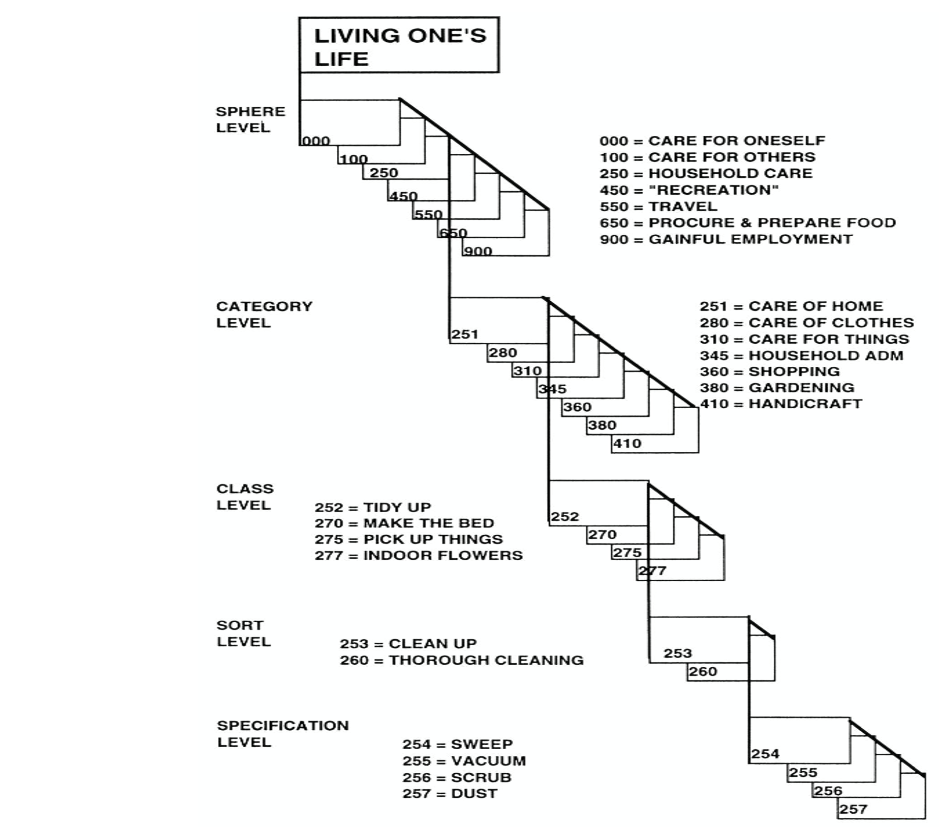
\includegraphics[width=0.45\linewidth]{fig3}
	\caption{An example of how the line from the sphere household care is organized into levels, with some alternatives at each level.} 
	\label{fig:Activity categorization scheme.}
\end{figure}
\hspace{1cm}These contexts reveal societal culture, individual preferences, and the interconnected nature of activities, goals, social interactions, and physical locations.The everyday context is shaped by an individual's rhythm of activities and societal timetables. The project context involves diverse activities tied to specific goals. The social context distinguishes between specialization and cooperation in household division of labor. The geographical context considers distances and location within the time-geographic method, with ongoing work to fully develop it.At the individual level, a rhythmic pattern emerges, emphasizing the significance of dwelling, workplace, and locations of friends, relatives, and shops. Geographical movement routines may vary, but the central role of places where friends and relatives reside remains consistent.[10]
\subsection{Leveraging Robotic Process Automation in the Management of Software Projects} 
\hspace{1cm}As technology advances rapidly, individuals and businesses are leveraging emerging trends for financial gains. One notable trend is Robot Process Automation (RPA). Market research from the future suggests that numerous industries stand to benefit from RPA, projecting a substantial market growth with a Compound Annual Growth Rate (CAGR) of 29 percent between 2017 and 2023. The impact of the pandemic in 2020 and 2021 has led to a significant surge in software usage. Modern software has become increasingly intricate, and development timelines have shortened due to heightened industry competition. Integrating robotic process automation into various aspects of software project management holds the potential to streamline repetitive tasks, reduce time constraints, and enhance overall organizational efficiency and productivity. This paper delves into specific areas within software project management where RPA can be applied to optimize processes effectively.[4]
\subsection{Managing  tasks} 

\subsubsection{Project Management}
\hspace{1cm}A project is a temporary endeavour with a defined beginning and end, undertaken to meet unique goals and objectives, typically to bring about beneficial change or added value. Project management involves the application of knowledge, skills, tools, and techniques to project activities to meet project requirements.Key aspects of project management include planning, organizing, controlling ,leading ,managing ,securing.Effective project management is crucial for delivering projects on time, within budget, and with the expected level of quality. Various methodologies and frameworks, such as Agile, Scrum, and Waterfall, are employed in project management to provide structured approaches to diverse types of projects.~\cref{fig:project management} 
 
\begin{figure}
	\centering
	\includegraphics[width=0.45\linewidth]{Fig1}
	\caption{Prioritizing tasks based on their dependency and urgency} 
	\label{fig:project management}
\end{figure}

\subsubsection{ Managing day-to-day task}
\hspace{1cm}Handling day-to-day tasks along with managing a project can be challenging, but effective time management and prioritization can make the process smoother. “Prioritization is a powerful skill that will help you take control of your workflow and optimize productivity.” Breaking your workload into manageable chunks and setting priorities helps you break the cycle of missed deadlines, last-minute rushes, and procrastination. ~\cref{fig:task management} While all the steps in prioritizing tasks are crucial, the most critical step is understanding how each task ranks in relation to your goals and objectives. By assessing the significance of tasks, you can prioritize effectively and ensure your efforts are directed toward activities that align with your overarching priorities.
 
\begin{figure}
	\centering
	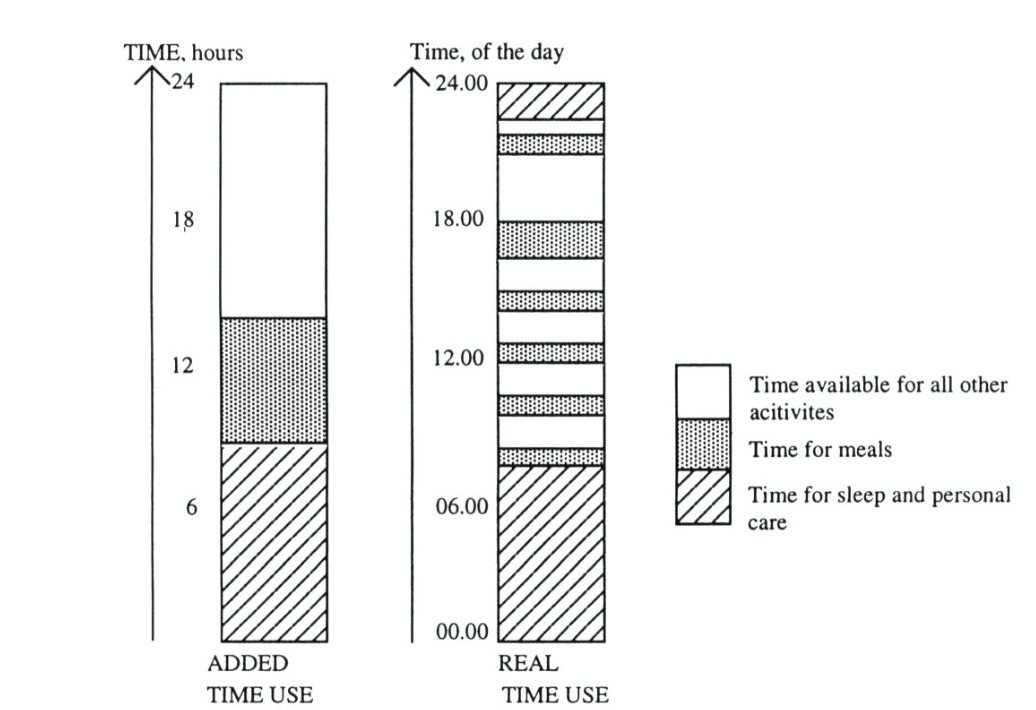
\includegraphics[width=0.45\linewidth]{fig2}
	\caption{Principal difference between added (left) and real (right) time-use.} 
	\label{fig:task management}
\end{figure}
\subsection{Technologies and tools involved in managing time and tasks}
\hspace{1cm}Tools and technologies play a crucial role in effectively managing the balance between everyday responsibilities and project management. These tools are specifically designed to address different aspects of the workload. Here's a breakdown of these tools based on their primary functions  for Time Management and Scheduling:Digital Calendars (e.g., Google Calendar, Microsoft Outlook): Perfect for organizing and tracking meetings, appointments, and deadlines.Time Tracking Applications (e.g., Toggl, Harvest): Excellent for recording time spent on various activities, aiding in workload management and capacity assessment.,Project Management:Task Management Platforms (e.g., Asana, Trello, Jira): Assist in organizing, prioritizing, and monitoring task and project progress.Gantt Chart Applications (e.g., Microsoft Project, Smartsheet): Useful for visualizing project schedules and understanding task interdependencies.Collaboration and Communication:Instant Messaging and Team Collaboration Tools (e.g., Slack, Microsoft Teams): Facilitate rapid communication and teamwork among project members,Video Conferencing Software(e.g., Zoom, Google Meet): Essential for conducting virtual meetings and staying in touch with team members and stakeholders,Document and FileManagement,Cloud-Based Storage (e.g., Google Drive, Dropbox, OneDrive): Essential for storing and sharing project-related documents and files.\\\hspace{1cm}Collaborative Document Editing Tools (e.g., Google Docs, Microsoft 365): Allow multiple users to simultaneously work on and edit documents,Resource Allocation and Delegation:Workload Assessment Tools (integrated within broader project management software): Help in analyzing and assigning tasks among team members.Outsourcing Platforms (e.g., Upwork, Fiverr): Useful for delegating tasks to external resources when necessary,Personal Productivity:Note-Taking Applications (e.g., Evernote, OneNote): Great for organizing personal notes, meeting minutes, and to-do lists.Mind Mapping Software (e.g., MindMeister): Aids in brainstorming and structuring ideas visually,Monitoring Workload and Employee Well-being:Employee Well-being Software (e.g., Officevibe, Culture Amp): Monitor team morale and individual stress levels to prevent burnout,Review and Reporting:Business Intelligence Tools (e.g., Tableau, Microsoft Power BI): Enable the creation of detailed reports on project progress and team performance.Each tool category plays a pivotal role in streamlining various aspects of task and project management, including scheduling, task allocation, collaboration, document management, and personal productivity. The right combination of these tools can significantly enhance efficiency and effectiveness in managing the balance between daily tasks and project responsibilities.
\newpage
 \vspace*{0.5cm}
 \section{Conclusion}
\hspace{1cm}In conclusion, the research offers valuable insights into the complexities of managing day-to-day tasks and projects, providing practical recommendations while acknowledging limitations. Further exploration and integration of suggested improvements in diverse organizational settings will contribute to evolving effective strategies in this dynamic landscape. The time-geographical approach analyzes daily life contexts, emphasizing interconnected activities at individual and household levels. It unveils societal culture and preferences, highlighting rhythmic patterns and central places. In software project management, leveraging Robotic Process Automation (RPA) is crucial for efficiency, with a projected market growth of 29 percentage  between 2017 and 2023. RPA integration can streamline tasks, reduce time constraints, and enhance overall productivity amid increased software usage due to the pandemic.
\newpage
 \vspace*{0.5cm}
\section{References} 
\bgroup\obeylines
\linespacing[1.66] 
 \hspace{1cm}[1] S. M. S. Islam and M. Rokonuzzaman, "Process centric work breakdown structure for easing Software Project management challenges: Business case analysis example," 2009 12th International Conference on Computers and Information Technology, Dhaka, Bangladesh, 2009, pp. 508-513, doi: 10.1109/ICCIT.2009.5407291
[2] S. Khan, S. Sharma, T. Singh and A. Juneja, "An Innovative Approach to Project Management and ePortals," 2023 International Conference on Computational Intelligence, Communication Technology and Networking (CICTN), Ghaziabad, India, 2023, pp. 359-363, doi: 10.1109/CICTN57981.2023.10140667.
[3] S. De and V. Vijayakumaran, "An Efficient Algorithm in Project Management for Resource Scheduling and Conflict Management using Graph Coloring Technique," 2020 IEEE International Conference for Innovation in Technology (INOCON), Bangluru, India, 2020, pp. 1-6, doi: 10.1109/INOCON50539.2020.9298193.
[4] C. Nitin Rajadhyaksha and J. R. Saini, "Robotic Process Automation for Software Project Management," 2022 IEEE 7th International conference for Convergence in Technology (I2CT), Mumbai, India, 2022, pp. 1-5, doi: 10.1109/I2CT54291.2022.9823972.
[5] V. Considine, "Systems engineering and strategic project management," IEE Half-Day Colloquium on Systems Engineering in Strategic Management Planning (Digest No: 1997/141), London, UK, 1997, pp. 2/1-2/4, doi: 10.1049/ic:19970779.
[6] R. Leano, S. Chattopadhyay and A. Sarma, "What makes a task difficult? An empirical study of perceptions of task difficulty," 2017 IEEE Symposium on Visual Languages and Human-Centric Computing (VL/HCC), Raleigh, NC, USA, 2017, pp. 67-71, doi: 10.1109/VLHCC.2017.8103452.
[7] M. Svahnberg and A. Karasira, "A Study on the Importance of Order in Requirements Prioritisation," 2009 Third International Workshop on Software Product Management, Atlanta, GA, USA, 2009, pp. 35-41, doi: 10.1109/IWSPM.2009.1.
[8] Hobday, M. (2000b). The project-based organisation: an ideal form for managing complex products and systems? Research Policy, 29(7–8), 871–893. https://doi.org/10.1016/s0048-7333(00)00110-4
[9] Khatib, M. E., Kherbash, A., Qassimi, A. A., Mheiri, K. A. (2022d). How can collaborative work and collaborative systems drive operational excellence in project management? Journal of Service Science and Management, 15(03), 297–307. https://doi.org/10.4236/jssm.2022.153017
[10] Ellegård, K. (1999). A time-geographical approach to the study of everyday life of individuals - a challenge of complexity. GeoJournal, 48(3), 167–175. http://www.jstor.org/stable/41147368


 

%***********************************References*********************************	 
\bibliographystyle{apacite}
\bibliography{References}
 
\end{document}
%%%%%%%%%%%%%%%%%%%%%%%%%%%%%%%%%%%%%%%%%%%%%%%%%%%%%%%%%%%%%%%%%%%%%%%%%%%%%%%%%%% 










